\documentclass{article}
\usepackage{fullpage}
\usepackage{graphicx}
\usepackage{url}
\begin{document}
\begin{centering}		
	\rule{\linewidth}{1mm} \\[0.5cm]
	{ \LARGE \bfseries ISyE 4803 - Foundations of Modern Data Science \\[0.2cm]
		Proposal}\\[0.5cm]
	\rule{\linewidth}{1mm} \\[1cm]
	
		\begin{tabular}{l p{5cm}}
		\textbf{Team Member Name:} & Austin Holt  \\
		\textbf{Project Title:} & Demand Prediction for Online Product Listings \\
		\end{tabular} 
\end{centering}

\vspace{2mm}

\section{Problem Statement}

In data science and machine learning, choosing the right model class is crucial. It can greatly affect the performance of predictive models. The model class chosen determines the complexity of the models, which affects their ability to find patterns in the data. However, the relationship between the size of the model class and the model’s performance can vary based on the dataset and the problem at hand.

This project aims to explore if increasing the model class size improves results for a specific dataset. The selected dataset for this problem is the Avito Demand Prediction dataset. It has features related to online classified listings, like text descriptions, images, and categorical variables. The target variable is the deal probability, which represents the likelihood of a listing leading to a successful transaction.

The main goal of this project is to evaluate the effect of model class size on the performance of models trained on this dataset. We’ll compare the performance of different model classes of varying sizes to see if larger model classes improve predictive accuracy. This understanding can help data scientists make informed decisions when choosing models for similar tasks. It can answer questions like whether it’s worth it to invest in larger, more complex models that are more expensive to train, or if simpler models can perform just as well.

\section{Data Source} 

The dataset used in this project is the Avito Demand Prediction dataset, which is sourced from a competition on Kaggle. Avito is a leading online classified platform in Russia, similar to Craigslist or eBay, where users can buy and sell a wide range of goods and services. The dataset contains information about online listings and the goal is to predict the deal probability, which represents the probability of a listing resulting in a successful transaction.

The dataset is provided in CSV and JPG format and consists of several files:

\begin{enumerate}
    \item train.csv: This file contains the training data, which includes various features of the listings along with the target variable, deal probability. It has 1,503,424 rows and 18 columns.
    \item test.csv: This file contains the test data, which includes the same features as the training data but without the target variable. It is used for making predictions and evaluating the performance of the trained models. It has 508,438 rows and 17 columns.
    \item train\_active.csv and test\_active.csv: These files contain supplementary information about the active listings during the training and testing periods, respectively. They include additional features such as the listing's activation date and the dates when the listing was displayed.
    \item train\_jpg.zip and test\_jpg.zip: These zip files contain the images associated with the listings in the training and test sets, respectively. Each image is identified by a unique image ID that corresponds to the 'image' column in the CSV files.
\end{enumerate}

The dataset encompasses a wide range of features describing a wide range of characteristics of the listings. Some of the key features include:

\begin{itemize}
    \item Title and description: The title and description text of the listing, which provide information about the product or service being offered.
    \item Category and subcategory: The hierarchical category structure of the listing, indicating the type of product or service.
    \item Price: The price of the listed item.
    \item Location: The geographical location of the listing, including the city and region.
    \item User information: Details about the user who created the listing, such as their ID and type (private or company).
    \item Image information: Metadata about the images associated with the listing, such as the image ID and a numerical representation of the image content.
\end{itemize}

The dataset used in this project was sourced from Avito and is publicly accessible via Kaggle. The dataset mirrors real-world situations where online platforms strive to estimate the probability of a successful transaction based on listing characteristics. The dataset’s extensive scope and its relevance to real-world scenarios make it a good choice for this investigation, enabling a comprehensive evaluation of various model classes and their capacity to discern the inherent patterns and relationships in the data.

\section{Methodology}


\subsection{Data Preprocessing}
The Avito Demand Prediction dataset was preprocessed to prepare it for model training and evaluation. Because test.csv did not contain the target 'deal\_probability', we elected to use a train/test split on the provided training data for the project. Due to the large size of train\_jpg.zip and hardware limitations, the images were unable to be utilized\footnote{After letting the computer extract train\_jpg.zip overnight, the author awoke to find that only 12\% progress had been made.}. For similar reasons, the rest of the dataset was randomly sampled down to 1,000 rows before proceeding to the preprocessing. The preprocessing steps included:
\begin{itemize}
\item Handling missing values: Missing values in categorical features were filled with the string 'missing', while missing values in numerical features were filled with 0.
\item Encoding categorical variables: Categorical features were encoded using LabelEncoder from scikit-learn, which assigns a unique numerical value to each category.
\item Scaling numerical features: Numerical features were scaled using StandardScaler from scikit-learn to have zero mean and variance one.
\item Text feature extraction: The 'title' and 'description' text features were transformed into numerical representations using TF-IDF vectorization with a maximum of 1000 features.
\end{itemize}
After preprocessing, the dataset was split into training and testing sets using an 80/20 split.



\subsection{Model Selection}
Several model classes were selected to evaluate their performance on the Avito Demand Prediction dataset:
\begin{itemize}
\item Constant Model: A baseline model that always predicts the mean deal probability of the training set.
\item K-Nearest Neighbors (KNN): A non-parametric model that predicts based on the average of the target values of the K nearest neighbors.
\item Linear Regression: A linear model that learns a linear combination of the input features to predict the target variable.
\item Lasso Regression: A linear model with L1 regularization to perform feature selection and prevent overfitting.
\item Ridge Regression: A linear model with L2 regularization to handle multicollinearity and prevent overfitting.
\item Neural Network: A multi-layer model with configurable hidden layers and activation functions able to represent highly complex functions.
\end{itemize}
These model classes were chosen to represent the main models covered throughout the course, covering a wide range of model class sizes and complexities. This variety allows for a comprehensive evaluation of the impact of model class size on predictive performance.


\subsection{Hyperparameter Tuning}
To ensure a fair comparison between the model classes, hyperparameter tuning was performed using grid search with cross-validation. The following hyperparameters were explored for each model class:
\begin{itemize}
   \item K-Nearest Neighbors (KNN):
   \begin{itemize}
       \item 'n\_neighbors': [5, 10, 20] - The number of neighbors to consider.
       \item 'weights': ['uniform', 'distance'] - The weight function used in prediction (uniform or distance-based).
   \end{itemize}
   
   \item Linear Regression:
   \begin{itemize}
       \item 'fit\_intercept': [True, False] - Whether to calculate the intercept for the linear model.
   \end{itemize}
   
   \item Lasso Regression:
   \begin{itemize}
       \item 'alpha': [0.1, 1.0, 10.0] - The regularization strength.
       \item 'max\_iter': [1000, 5000, 10000] - The maximum number of iterations for the solver.
   \end{itemize}
   
   \item Ridge Regression:
   \begin{itemize}
       \item 'alpha': [0.1, 1.0, 10.0] - The regularization strength.
   \end{itemize}
   
   \item Neural Network (Multi-layer Perceptron):
   \begin{itemize}
       \item 'hidden\_layer\_sizes': [(100,), (200,), (100, 100), (200, 200), (100, 100, 100), (200, 200, 200)] - The number and size of hidden layers.
       \item 'activation': ['relu', 'tanh'] - The activation function for the hidden layers.
       \item 'solver': ['adam', 'sgd'] - The solver for weight optimization.
   \end{itemize}
\end{itemize}

Grid search with 5-fold cross-validation was used to search through all possible combinations of the specified hyperparameters for each model class. The objective was to find the best hyperparameter configuration that minimizes the root mean squared error (RMSE) on the validation sets.

The choice of hyperparameter values was based on commonly used ranges and values for each model class. For example:
\begin{itemize}
   \item For KNN, the number of neighbors was varied from a small value (5) to larger values (10 and 20) to capture different neighborhood sizes. The weight function was set to either 'uniform' (equal weights) or 'distance' (weights inversely proportional to distance) to account for different weighting schemes.
   \item For linear regression, the 'fit\_intercept' parameter was set to either True or False to determine whether to include the intercept term in the model.
   \item For lasso and ridge regression, the regularization strength ('alpha') was varied from small (0.1) to large (10.0) values to control the amount of regularization applied. For Lasso Regression, the maximum number of iterations ('max\_iter') was also tuned to ensure convergence.
   \item For the neural network, the architecture was varied by considering different numbers and sizes of hidden layers, ranging from a single hidden layer with 100 or 200 neurons to multiple hidden layers with varying sizes. The activation function for the hidden layers was set to either 'relu' (rectified linear unit) or 'tanh' (hyperbolic tangent) to introduce non-linearity. The solver for weight optimization was chosen between 'adam' (adaptive moment estimation) and 'sgd' (stochastic gradient descent).
\end{itemize}

By exploring these hyperparameter spaces, the grid search aims to find the optimal configuration for each model class that maximizes its predictive performance on the dataset. The best hyperparameters found through cross-validation were then used to train the final models on the entire training set and evaluate their performance on the test set.


The trained models were evaluated on the test set using root mean square error (RMSE). RMSE measures the average squared difference between the predicted and actual deal probabilities. Lower RMSE indicates better predictive performance. Cross-validation scores and test set performance were reported for each model class to assess their predictive accuracy and generalization ability.


\subsection{Model Comparison}
The performance of the different model classes was compared based on their cross-validation scores and test set metrics. The relationship between model class size and predictive performance was analyzed to determine if increasing model complexity yields meaningful improvements.

Additionally, the results were visualized using bar plots to provide a clear comparison of the model classes' performance. The plots included the test set RMSE for all models and a separate plot excluding the linear regression model to better visualize the performance differences among the other models\footnote{The first plot is heavily skewed by the linear regression's RMSE and does not provide meaningful insight as a result. Because of this, it will not be shown in this paper but is still accessible in the Jupyter notebook.}.


\section{Evaluation and Final Results}

The performance of the different model classes was evaluated using cross-validation scores and test set metrics. The cross-validation scores provide an estimate of the model's performance on unseen data, while the test set metrics give a final assessment of the model's predictive accuracy.

Table \ref{tab:results} presents the cross-validation scores and test set metrics for each model class.

\begin{table}[ht]
\centering
\begin{tabular}{|l|c|c|}
\hline
\textbf{Model Class} & \textbf{CV Score (RMSE)} & \textbf{Test RMSE} \\
\hline
Constant & 0.2156 & 0.2056 \\
KNN & 0.2153 & 0.1948 \\
Linear Regression & 1.5335 & 21.1043 \\
Lasso Regression & 0.2111 & 0.2023 \\
Ridge Regression & \textbf{0.2015} & \textbf{0.1916} \\
Neural Network & 0.2195 & 0.2098 \\
\hline
\end{tabular}
\caption{Cross-validation scores and test set metrics for each model class.}
\label{tab:results}
\end{table}

The ridge regression achieved the best performance, with the lowest cross-validation score and test set RMSE. The KNN model also performed well, outperforming the other models. The constant model baseline also did well, outperforming the neural network. The linear regression performed poorly on this dataset, with RMSE scores indicating that on average, it didn't even predict values between 0 and 1.

To visualize the performance differences between the model classes, Figure \ref{fig:test_rmse} displays a bar plot of the test set RMSE for each model.

\begin{figure}[ht]
\centering
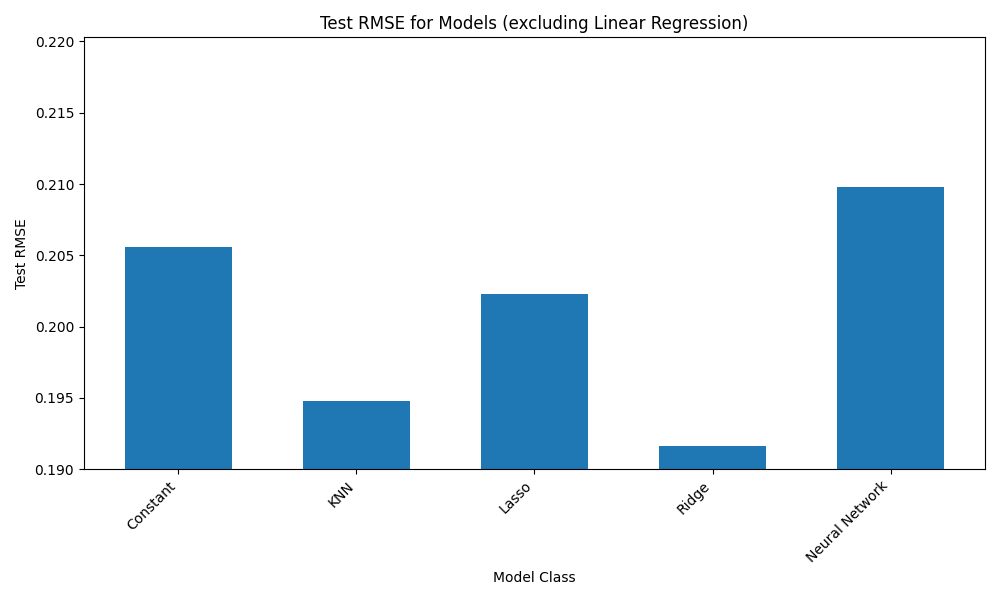
\includegraphics[width=0.8\textwidth]{test_rmse_plot_no_linear.png}
\caption{Bar plot of test set RMSE for each model class, excluding linear regression.}
\label{fig:test_rmse}
\end{figure}

The plot shows the superiority of the ridge regression and KNN models compared to the other model classes. The lasso regression model performed slightly better than the constant model, while the neural network had the highest RMSE\footnote{Excluding the linear regression.}.

Interestingly, the test RMSE plot does not show a clear correlation between model complexity and performance. The ridge regression achieved the best performance, while the more complex neural network did not lead to better performance compared to simpler models like KNN and lasso. This suggests that, at least for this dataset, increasing model complexity does not guarantee improved predictive performance.

While the evaluation results provide certain insights on model selection, it is important to acknowledge potential sources of error. One source of error could be the limited size of the dataset used in this project. Due to computational constraints, a subset of the original dataset was used, reducing the number of data points available for the models to capture. Additionally, the preprocessing steps, such as handling missing values and encoding categorical variables, could introduce some level of error or bias. The choice of hyperparameters for each model class, although tuned using grid search, may not be fully exhaustive and could potentially impact the results. Furthermore, the evaluation metric (RMSE) while commonly used, may not capture all aspects of model performance and may be sensitive to certain characteristics of the target feature. It is crucial to consider these potential sources of error when interpreting the results and drawing conclusions from this project.

	\pagebreak

\section{References}

Kaggle. (n.d.). Avito Demand Prediction . Retrieved from 

\url{https://www.kaggle.com/c/avito-demand-prediction}

\end{document}

